\item \textbf{{[}RVHS/PRELIM/9569/2021/P2/Q1{]} }

\textbf{Task 1.1}

Write a function \texttt{task1\_1(name\_A, name\_B)} where \texttt{name\_A}
and \texttt{name\_B} are strings which consists of only alphabet letters
and spaces. The function will return \texttt{True} if 
\begin{itemize}
\item the alphabet letters combination used in string \texttt{name\_A} and
\texttt{name\_B} are the same and
\item the spaces in string \texttt{name\_A} and \texttt{name\_B} are at
the same locations. \hfill{}{[}7{]}
\end{itemize}
For example, 

\noindent %
\noindent\begin{minipage}[t]{1\columnwidth}%
\texttt{>\textcompwordmark >\textcompwordmark > match\_names(\textquotedbl Abcde\textquotedbl ,
\textquotedbl Deabc\textquotedbl ) }

\texttt{True }

\texttt{>\textcompwordmark >\textcompwordmark > match\_names(\textquotedbl Abcde
Fgh I\textquotedbl , \textquotedbl Ihgfe Dcb A\textquotedbl ) }

\texttt{True }

\texttt{>\textcompwordmark >\textcompwordmark > match\_names(\textquotedbl Abcd
Efgh I\textquotedbl , \textquotedbl Ihgfe Dcb A\textquotedbl ) }

\texttt{False }

\texttt{>\textcompwordmark >\textcompwordmark > match\_names(\textquotedbl Abcde
Fzh I\textquotedbl , \textquotedbl Ihgfe Dcb A\textquotedbl ) }

\texttt{False} %
\end{minipage}

Test your program with the following test data: 

\noindent\begin{minipage}[t]{1\columnwidth}%
\texttt{print(task1\_1(\textquotedbl Abcde\textquotedbl , \textquotedbl Deabc\textquotedbl )) }

\texttt{print(task1\_1(\textquotedbl Abcde Fgh I\textquotedbl ,
\textquotedbl Ihgfe Dcb A\textquotedbl )) }

\texttt{print(task1\_1(\textquotedbl Abcd Efgh I\textquotedbl ,
\textquotedbl Ihgfe Dcb A\textquotedbl )) }

\texttt{print(task1\_1(\textquotedbl Abcde Fzh I\textquotedbl ,
\textquotedbl Ihgfe Dcb A\textquotedbl ))}%
\end{minipage} 

\subsubsection*{Task 1.2 }

Write the function \texttt{task1\_2()} to read the names in file \texttt{\textquotedbl namelist\_A.txt\textquotedbl}
and find a matching name in \textquotedbl\texttt{namelist\_B.txt}\textquotedbl{}
that satisfied the conditions stated in \textbf{Task 1.1}. If a matching
name cannot be found in \textquotedbl\texttt{namelist\_B.txt}\textquotedbl ,
it will just display \textquotedbl\texttt{{*}{*}{*}{*}{*}{*}{*}{*}{*}{*}{*}No
match{*}{*}{*}{*}{*}{*}{*}{*}{*}{*}{*}}\textquotedbl . Your results
should be displayed in the following manners. The time-complexity
of your program code matters. \hfill{}{[}13{]}
\begin{center}
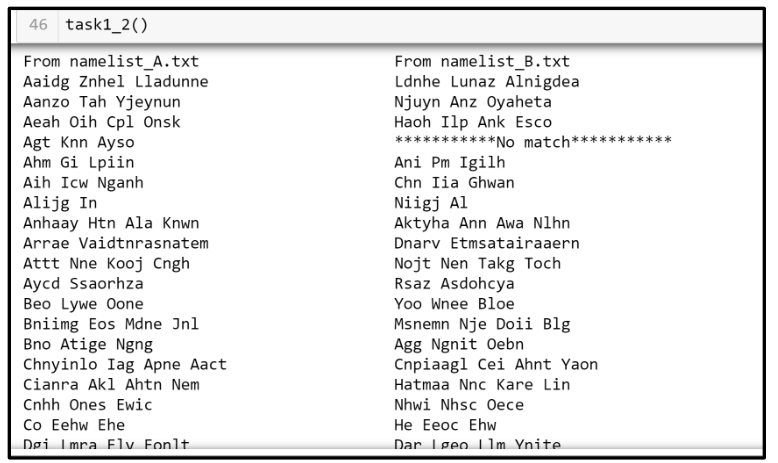
\includegraphics[width=0.5\paperwidth]{C:/Users/Admin/Desktop/Github/question_bank/LyX/static/img/9569-RVHS-2021-P2-Q1}
\par\end{center}